%%%%%%%%%%%%%%%%%%%%%%%%%%%%%%%%%%%%%%%%%
% Journal Article
% LaTeX Template
% Version 1.4 (15/5/16)
%
% This template has been downloaded from:
% http://www.LaTeXTemplates.com
%
% Original author:
% Frits Wenneker (http://www.howtotex.com) with extensive modifications by
% Vel (vel@LaTeXTemplates.com)
%
% License:
% CC BY-NC-SA 3.0 (http://creativecommons.org/licenses/by-nc-sa/3.0/)
%
%%%%%%%%%%%%%%%%%%%%%%%%%%%%%%%%%%%%%%%%%

%----------------------------------------------------------------------------------------
%	PACKAGES AND OTHER DOCUMENT CONFIGURATIONS
%----------------------------------------------------------------------------------------

\documentclass[twoside,twocolumn]{article}

\usepackage{blindtext} % Package to generate dummy text throughout this template 

\usepackage[sc]{mathpazo} % Use the Palatino font
\usepackage[T1]{fontenc} % Use 8-bit encoding that has 256 glyphs
\linespread{1.05} % Line spacing - Palatino needs more space between lines
\usepackage{microtype} % Slightly tweak font spacing for aesthetics

\usepackage[english]{babel} % Language hyphenation and typographical rules

\usepackage[hmarginratio=1:1,top=32mm,columnsep=20pt,left=2cm,right=2cm,top=2cm,bottom=2cm]{geometry} % Document margins
\usepackage[hang, small,labelfont=bf,up,textfont=it,up]{caption} % Custom captions under/above floats in tables or figures
\usepackage{booktabs} % Horizontal rules in tables

\usepackage{lettrine} % The lettrine is the first enlarged letter at the beginning of the text

\usepackage{enumitem} % Customized lists
\setlist[itemize]{noitemsep} % Make itemize lists more compact

\usepackage{abstract} % Allows abstract customization
\renewcommand{\abstractnamefont}{\normalfont\bfseries} % Set the "Abstract" text to bold
\renewcommand{\abstracttextfont}{\normalfont\small\itshape} % Set the abstract itself to small italic text

\usepackage{titlesec} % Allows customization of titles
\renewcommand\thesection{\Roman{section}} % Roman numerals for the sections
\renewcommand\thesubsection{\roman{subsection}} % roman numerals for subsections
\titleformat{\section}[block]{\large\scshape\centering}{\thesection.}{1em}{} % Change the look of the section titles
\titleformat{\subsection}[block]{\large}{\thesubsection.}{1em}{} % Change the look of the section titles

\usepackage{fancyhdr} % Headers and footers
\pagestyle{fancy} % All pages have headers and footers
\fancyhead{} % Blank out the default header
\fancyfoot{} % Blank out the default footer
\fancyhead[C]{Running title $\bullet$ May 2016 $\bullet$ Vol. XXI, No. 1} % Custom header text
\fancyfoot[RO,LE]{\thepage} % Custom footer text

\usepackage{titling} % Customizing the title section

\usepackage{hyperref} % For hyperlinks in the PDF

% Packages maison
\usepackage{amsmath,amssymb} % For including math equations, theorems, symbols, etc
\usepackage{bm}
\usepackage{graphicx} % Required for including images
\graphicspath{{../Figures/}} % Set the default folder for images
\usepackage{prettyref}

%----------------------------------------------------------------------------------------
%	TITLE SECTION
%----------------------------------------------------------------------------------------

\setlength{\droptitle}{-4\baselineskip} % Move the title up

\pretitle{\begin{center}\Huge\bfseries} % Article title formatting
\posttitle{\end{center}} % Article title closing formatting
\title{A database of piano and orchestral midi scores.\\Application to automatic projective orchestration} % Article title
\author{%
\textsc{John Smith}\thanks{A thank you or further information} \\[1ex] % Your name
\normalsize University of California \\ % Your institution
\normalsize \href{mailto:john@smith.com}{john@smith.com} % Your email address
%\and % Uncomment if 2 authors are required, duplicate these 4 lines if more
%\textsc{Jane Smith}\thanks{Corresponding author} \\[1ex] % Second author's name
%\normalsize University of Utah \\ % Second author's institution
%\normalsize \href{mailto:jane@smith.com}{jane@smith.com} % Second author's email address
}
\date{\today} % Leave empty to omit a date
\renewcommand{\maketitlehookd}{%
\begin{abstract}
\noindent This article introduces the \textbf{NAME} dataset, a freely-available collection of midi scores 

midi score database. It is composed by (137 OU 224 si IMSLP, mais c'est tout faux) pairs of one piano score and one corresponding orchestration. To our best knowledge, this is the first database of this kind. Thus, we also introduce a projective orchestration task, which roughly consists in learning to perform automatic orchestration of a piano score. This task can be addressed using learning methods on this database.  
\end{abstract}
}

%----------------------------------------------------------------------------------------

\begin{document}

% Print the title
\maketitle

%----------------------------------------------------------------------------------------
%	ARTICLE CONTENTS
%----------------------------------------------------------------------------------------

\section{Introduction}
% Orchestration = definition
Orchestration is the subtle art of writing musical pieces for the orchestra by combining the properties of various instruments in order to achieve a particular sonic rendering. \cite{koechli_orch,Rimsky-Korsakov:1873aa}. 
% Orchestration projective
Among the different writing techniques for orchestration, we define \textit{projective orchestration} as the technique which consists in writing first a piano score and then projecting it on an orchestra. This technique has been long used by classic composers \textbf{(exemple ?)}.
% Dataset symbolic pour l'orchestration projective
This paper introduces what is to our best knowledge, the first symbolic dataset of projective orchestration.
% Rapide description
It contains midi scores of piano pieces, and for each of this piece, one or several corresponding orchestration(s) written by famous composers.

This database has several purposes :
\begin{itemize}
\item being the starting point for a scientific investigation of orchestration, especially for statistic-based approaches on high-level symbolic information
\item establishing a reference dataset for generative algorithms 
\item indexing works of famous composers for musicological purposes
\end{itemize}

The remainder of this paper is organized as follows. The first section introduces the structure of the database, the reason why it has been created and how informations have been gathered. In the section two, we introduce an automatic projective orchestration task. Our proposed algorithm rely on learning based methods, and uses this database. We also define an evaluation criterion that uses a part of the database. Conclusions are provided in the last section.

\section{Dataset}
\subsection{Symbolic information for orchestration}
% Teahching orchestration = exemples
Several treatise of orchestration exist \cite{koechli_orch,piston-orch,Rimsky-Korsakov:1873aa}, but they all consist in a sum of examples rather than a comprehensive theorization.
% Why ? Because it is highly complex, and we can't handle this complexity
An explanation of this observation lies in the tremendous complexity that emerges from an orchestral work. For the composer, the number of pitch and intensity ranges of each instrument is powered by the number of instruments in the orchestra, and lead to a huge combinatoric. During the performance, acoustic summation of the instruments give rise to highly non-linear effects at the signal level, which make the resulting sound almost impossible to predict. Eventually, only a little is known about the complex psycho-acoustic phenomena involved in the listening process. All those aspects play an important role in an orchestral work. Then, it seems almost impossible for a human mind to grasp in its entirety an orchestral rendering.

% Problem too complex : need for scientific investigation
Hence, we believe that a thorough scientific investigation could help disentangling the multiple factors involved in an orchestral work, and might be a precious help toward a greater understanding of the discipline.
% Scientific investigation already made ? Yes : signal et psycho-ac
If major works have already been produced in psycho-acoustic CITE and signal processing CITE, no attempts have been made to tackle orchestration from a symbolic perspective.
Here, symbolic means a scores with musical notation, as represented in \ref{fig:orch}.
% Utilité du symboliques
However, symbolic representations convey high-level information. Observing famous orchestral works from this perspective could be gratifying.
% Pourquoi pas de symbolique alors ? Complexité + pas encore les techniques adaptées
The combinatorial complexity involved by symbolic representation is directly related to the average pitch range of an instrument powered by the number of instrument. For a symphonic orchestra, we see that this complexity quickly explode. Even for a computer, an exhaustive investigation of all the possible combinations is unimaginable.
% Et maintenant on a le deep learning
But the recent advent in machine learning brought techniques that could cope with the dimensionality involved by symbolic data.
% Mais on a besoin de... DATA :)
Based on statistical tools, those techniques require a huge amount of data. This dataset is a first attempt to fill this gap.

\begin{figure}
\centering
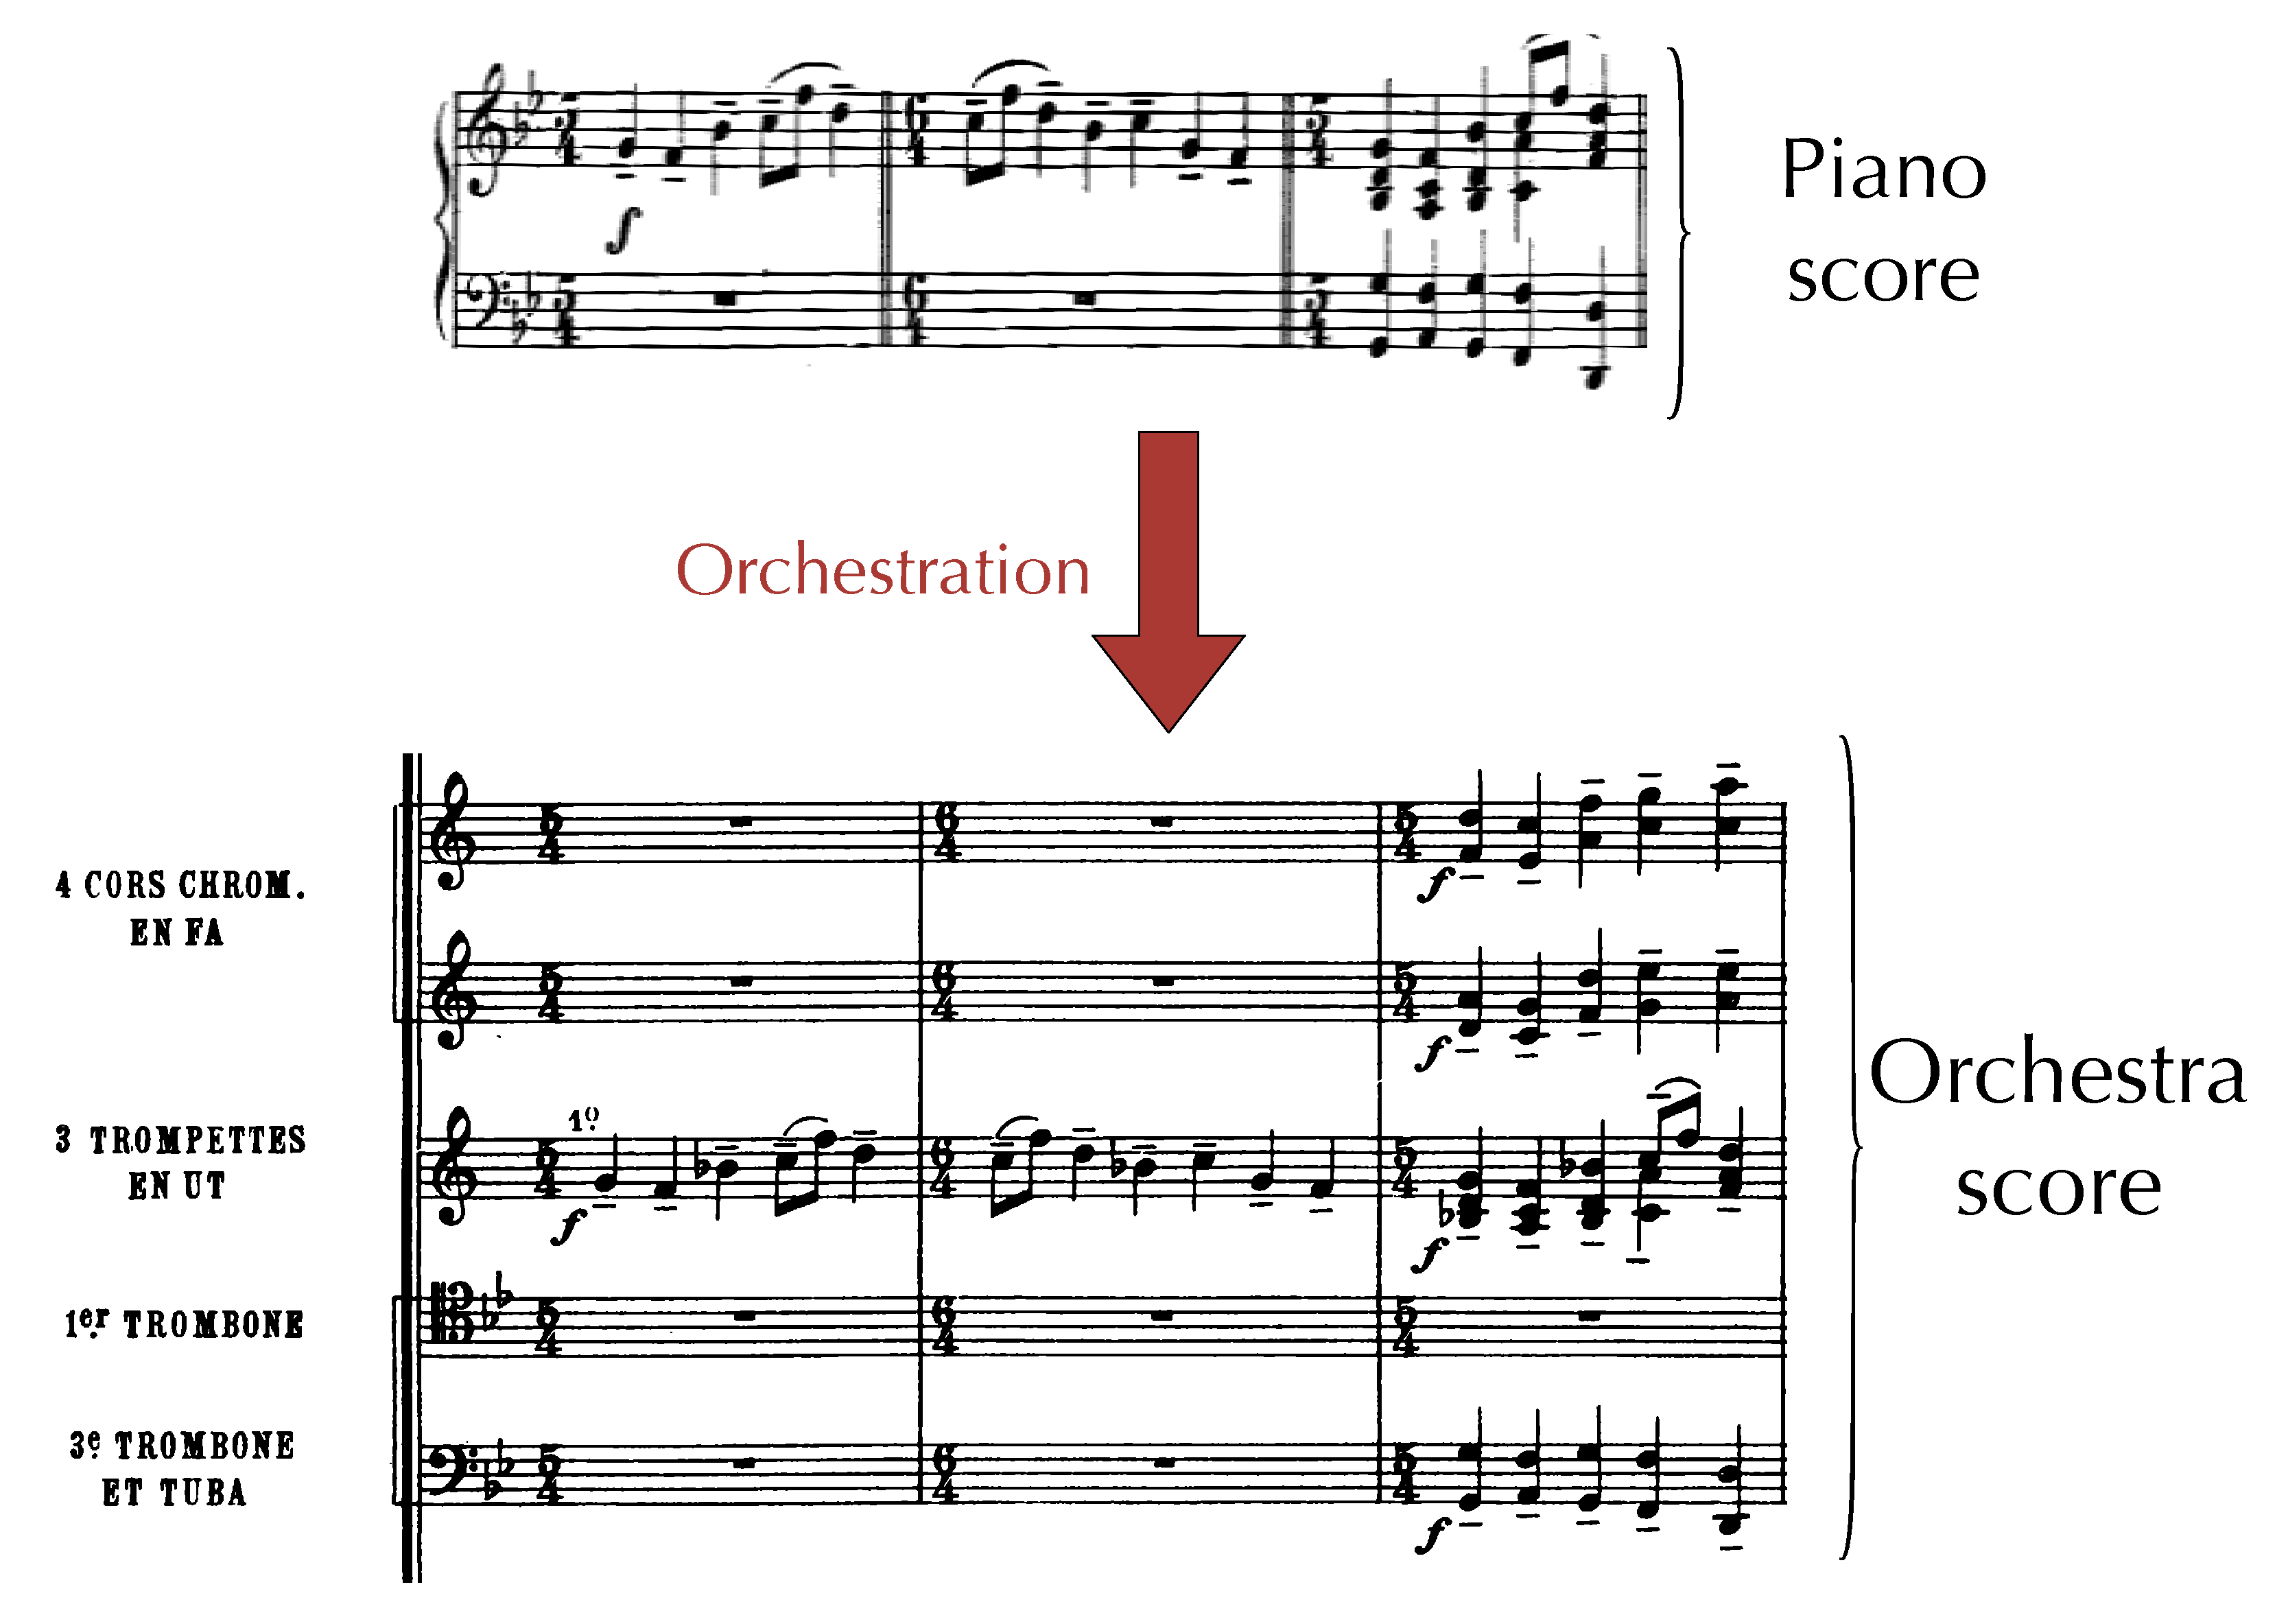
\includegraphics[scale=0.12]{orch}
\caption{\textit{Projective orchestration}. A piano score is projected on an orchestra. Even though a wide range of orchestrations exist for a given piano score, all of them will share strong relations with the original piano score. One given orchestration implicitly embeds the knowledge of the composer about timbre and orchestration.}
\label{fig:orch}
\end{figure}

\subsection{Why projective orchestration}
% Pourquoi c'est intéressant les orchestrations projectives ?
We think that projective orchestration is an extremely interesting particular case. Because orchestrating a piano piece often stem from its analysis, studying the orchestration written by a famous composer is, in a restricted way, listening to its analysis. Besides, the harmonic, rhythmic and melodic structure of a piece is already fixed in the piano score, and observing the joint information of the original piano score and an orchestrated version consists in focusing on the timbral augmentation of this primal structure. In other words, it allows to focus on how the musical discourse is highlighted by the evolution of the timbre.

\subsection{Structure of the database}
% Number of file, main aspect a+ Format midi
The \textbf{NAME} database consists in piano and orchestra scores in MIDI format. 
% Organization, hierarchy
The files are grouped in folders indexed by a number. Each folder contains a pair : piano score and a possible orchestration. 
% Where does it come from
Since the files have been manually collected on several existing databases on the internet,
% CSV instrumentation
the relation between the track name and the instrument this track effectively represents is often not obvious. For that reason, a \textit{CSV} file is associated to each \textit{MIDI} file. It has the same name as the midi file. It links the name of the track in the midi file and the name of an instrument, according to a nomenclature (see nomenclatura.txt at the root of the folder).
% Metadata
% Aligned and non-aligned versions
% Other statistics

\subsection{Alignment algorithm}
Since we gathered files from various origins, we had to perform automatic alignment for each pair. We used a \textit{Needleman-Wunsch} based algorithm with a measure adapted to the musical context.

\section{A case study : projective automatic orchestration}

%------------------------------------------------

\section{Projective orchestration}


%----------------------------------------------------------------------------------------
%	REFERENCE LIST
%----------------------------------------------------------------------------------------

\bibliographystyle{plain}
\bibliography{../Biblio/biblio}

%----------------------------------------------------------------------------------------

\end{document}
